\documentclass{standalone}
\usepackage{tikz}

\usetikzlibrary{math}


\begin{document}

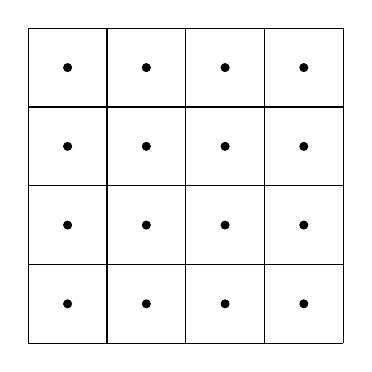
\begin{tikzpicture}
  \draw (0,0) grid (4,4);

  \foreach \i in {1,2,3,4} {
    \foreach \j in {1,2,3,4} {
      \tikzmath{
        real \x;
        real \y;
        \x = \i - 0.5;
        \y = \j - 0.5;
      }

      \draw[fill=black] (\x, \y) circle [radius=0.05cm];
    }
  }
\end{tikzpicture}

\end{document}